%%%%%%%%%%%%%%%%%%%%%%%%%%%%%%%%%% BIBLIOTHEQUES %%%%%%%%%%%%%%%%%%%%%%%%%%%%%%%%%
\documentclass[12pt , a4paper,titlepage]{report}
\usepackage[francais]{babel}
\usepackage[T1]{fontenc}
\usepackage[utf8]{inputenc}
\usepackage{lmodern,textcomp}
%Pour l'index
\usepackage{makeidx}
\makeindex
\usepackage{graphicx}
\usepackage{color}
\definecolor{gris}{gray}{0.75}

%%%%%%%%%%%%%%%%%%%%%%%%%%%%%%%%%% PAGE DE GARDE %%%%%%%%%%%%%%%%%%%%%%%%%%%%%%%%%

\begin{document}
\pagecolor{gris}
\begin{titlepage}
\begin{figure}
  \begin{flushright}
   \begin{minipage}[c]{0.25\linewidth}
      
\includegraphics[width=0.5\linewidth]{IUT-Orleans.jpg}
   \end{minipage}
   \end{flushright}
 	\begin{flushleft}
		\small Antoine GELOT\\
		\small Arthur LETORT \\
		\small Dimitri LEDOUARIN \\
		\small Florian LE CORRE \\
		\small Thomas MALFILATRE \\
	\end{flushleft}
\end{figure}
     
\title{\Huge {\textbf  { Projet tutoré: Puits canadien}}
	\begin{center}
		\bigskip
		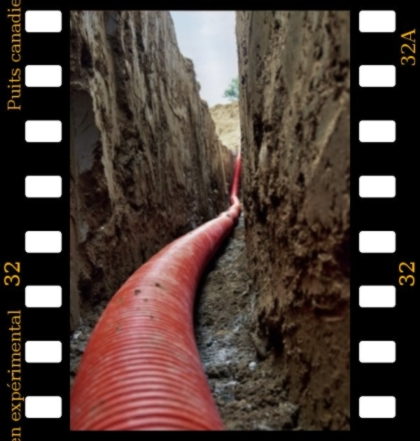
\includegraphics[width=10cm, height=6cm]{PC.jpg}
	\end{center}
}



\date{\begin{flushleft}
\vfill 2e année DUT Informatique : 2012 - 2013 \end{flushleft} 
}
\end{titlepage}

%%%%%%%%%%%%%%%%%%%%%%%%%%%%%%%%%%% DEVELOPPEMENT %%%%%%%%%%%%%%%%%%%%%%%%%%%%%%%%%


\maketitle

\begin{center}

\bf \huge \bigskip \bigskip Remerciements 
\end{center}

 \bigskip \bigskip \bigskip \bigskip \bigskip  \bigskip \bigskip 
\paragraph{Avant de commencer ce rapport nous tenions à remercier Monsieur Escot ainsi
 que Monsieur Jubertie pour leur soutien qu'ils nous ont apporté. En effet les différentes réunions organisées nous ont
  permis de mieux comprendre le fonctionnement du projet.}
\paragraph {Ce projet a eu un impact sur notre fin de formation. Il a permis la jonction entre l'IUT et la vie professionnelle en y
 ayant acquis un véritable sens coopératif afin de mieux nous insérer au sein d'un stage en entreprise.}


\tableofcontents


%%%%%%%%%%%%%%%%%%%%%%%%%%%%%%%%%%% INTRO %%%%%%%%%%%%%%%%%%%%%%%%%%%%%%%%%

 \chapter{Introduction}
 \paragraph{   L'année dernière le projet du puits canadien avait été confié à des étudiants pour permettre une récupération des données
 via une carte Arduino pour les mettre sur un site internet. }
 \paragraph{   Pour cette année, les professeurs voulaient désormais un site internet avec une représentation du puits canadien en 3D, 
 plutôt que le 2D qui était peu intuitif, pour pouvoir se repérer et se déplacer dans le puits canadien.}
 \paragraph{   Nous nous sommes donc concentrés sur cette représentation 3D et avons laissé de côté la partie Arduino qui était plutôt
 secondaire et déjà réalisé l'année dernière.}


%%%%%%%%%%%%%%%%%%%%%%%%%%%%%%%%%%% CHAP 1 %%%%%%%%%%%%%%%%%%%%%%%%%%%%%%%%%

 \chapter {Le site internet}
 \section{Choix des bibliothèques}
 \subsection{Pour la 3D}
 \paragraph{Pour réaliser la modélisation 3D du puits canadien, nous avons décidé d'utiliser la bibliothèque THREE.JS, qui est simple
 d'utilisation et permet de faire plusieurs modèles en 3D.}
 \paragraph{ Cette bibliothèque nous a donc permis de créer le puits canadien et d'y ajouter les sondes pour mieux comprendre leurs 
 emplacements. On peut également zoomer,dézoomer, faire pivoter le puits grâce à l'implémentation de THREE.JS. }
 \begin{center}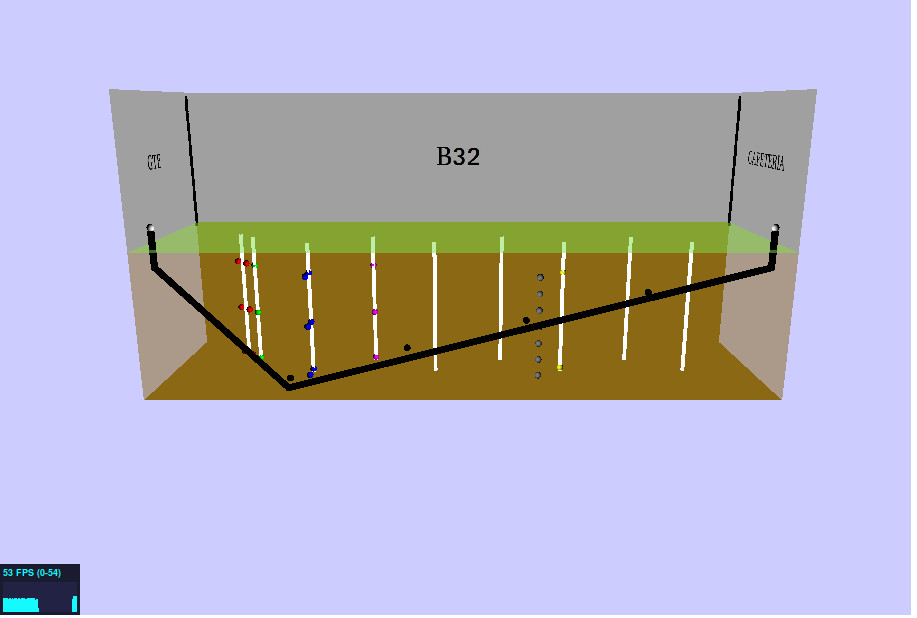
\includegraphics[width=10cm]{puit.jpg}\end{center}
 \subsection{Pour les graphes}

 \paragraph{   En ce qui concerne le graphe pour récupérer les températures et autres données, nous avons utilisé la bibliothèque déjà 
 présente "HIGHCHARTS". }
 \paragraph{   Nous avons décidé de garder HIGHCHARTS car cette bibliothèque était déjà implémentée et elle permet de réaliser des
 graphes de qualités.}
 \paragraph{  Cette bibliothèque nous permet aussi de zoomer sur une partie de graphe. On peut également facilement le graphe en
 différents formats (PNG,JPEG,PDF ou SVG).} 
 \begin{center}
    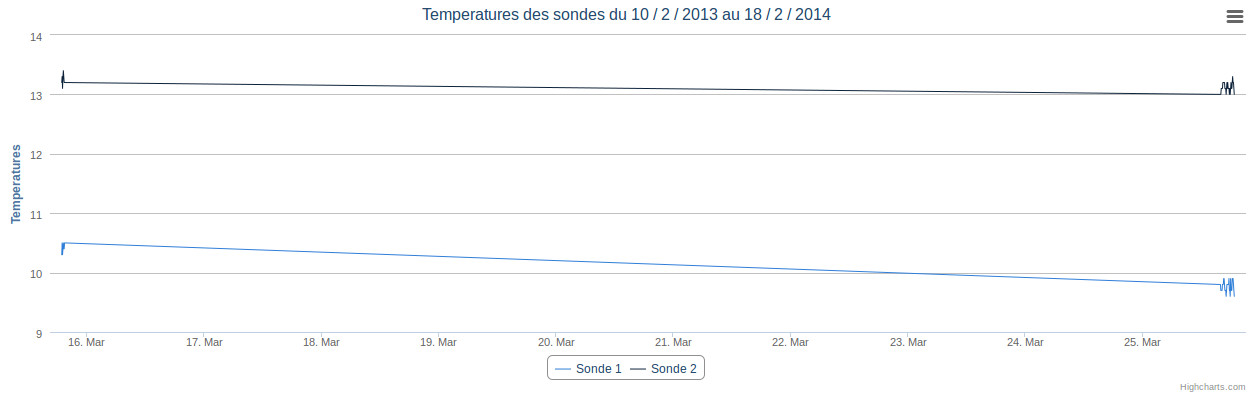
\includegraphics[width=15cm, height=10cm]{temperature.jpg}
 \end{center}
  \newpage
 \section{L'implémentation de THREE.JS}
 \paragraph{   Etant donné qu'HIGHCHARTS était déjà implémentée, l’implémentation de Three a été plutôt simple à réaliser. Three étant 
 aussi une bibliothèque javascript comme HIGHCHARTS, il a fallu réaliser le transfert de données javascript en php.}
 \paragraph{Le php permet d’établir la connexion avec la base de données et
ainsi pouvoir récupérer toutes les données nécessaires à afficher. Nous avons donc eu donc quelques difficultés à faire passer le 
javascript en php.}
 \paragraph{Cela nous a posé des problèmes, notamment pour le passage au niveau du graphe des températures mais nous avons finalement
 trouvé la solution.}
 
 \section {Disposition des menus}
 \begin{center} 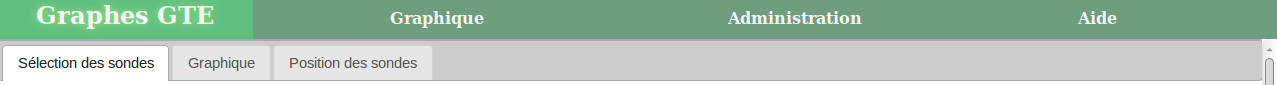
\includegraphics[width=16.5cm]{menu.jpg}\end{center}
 \paragraph {   Nous avons décidé de laisser le site séparé en trois parties en opérant quelques changements: }
 \begin{itemize}
 \item Une contenant les graphiques. Elle contient elle même trois sous menu permettant de choisir le type de graphe voulu. 
 Le premier menu permet de voir la modélisation du puits canadien en 3D et de ses sondes, et de générer le deuxième sous menu. 
  Le deuxième permet d'avoir la température en fonction des sondes  et des dates sélectionnées préalablement.
   Enfin, le troisième onglet montre une image permettant de mieux situer les sondes et corbeilles dans un schéma 2D.
 \item Une pour l’administration, qui permet à l'utilisateur,à condition d'avoir le mot de passe,
  d’interagir avec la base de données via des formulaires d'ajout, de suppression,etc...
 \item Une pour l’aide, qui explique comment utiliser les différentes fonctionnalités du site.
 \end{itemize}


%%%%%%%%%%%%%%%%%%%%%%%%%%%%%%%%%%% CHAP 2 %%%%%%%%%%%%%%%%%%%%%%%%%%%%%%%%%

 \chapter{La base de données}
 \section{Ajout de propriétés}
 
 \paragraph{ Nous avons repris la même base de données du projet de l'année dernière, cependant nous avons rajouté différentes propriétés demandés 
par Mr Escot.}
	\begin{itemize}
		\item Pour les sondes
		\begin{itemize}
			\item Les positions x,y,z pour les placer correctement dans la représentation 3D du puits canadien.
		\end{itemize}
		\item Pour les corbeilles
		\begin{itemize}
			\item Les positions x,y,z pour les placer correctement dans la représentation 3D du puits canadien.
			\item Les noms des corbeilles ont été changé pour permettre l'appartenance d'une sonde à une corbeille qui était mal géré. 
		\end{itemize} 
	\end{itemize}
 \paragraph{   Ces ajouts de propriétés nous ont donc permis de mieux gérer la base de données et ainsi les différents graphes.  }
 \section{Administration}
	\paragraph{En ce qui concerne la partie Administration du site internet, il faut y rentrer à l'aide d'un mot de passe prédéfini. Ensuite, on
	peut ajouter ou supprimer tous types d'éléments en sélectionnant le menu que l'on souhaite. L'élément sera automatiquement ajouté dans la base 
	de données et affiché sur la représentation 3D du puits canadien.}
%%%%% IMAGE DE LA PARTIE ADMINISTRATION %%%%%%
 \section{Import/Export}
 \paragraph{   Grâce à l'onglet d'import/export, il est possible de sauvegarder les données par l'export, dans un fichier. La base de 
 données actuelle enregistrée est sauvegardée sous un format SQL.}
 \paragraph{   Par ailleurs, l'import permettra l'initialisation de la base de donnée à un état préalable. C'est à dire que nous 
 pouvons mettre la base de données à l'égale d'une ancienne version exportée.} 




%%%%%%%%%%%%%%%%%%%%%%%%%%%%%%%%%%% CHAP 3 %%%%%%%%%%%%%%%%%%%%%%%%%%%%%%%%%

 \chapter{Organisation}
 \section{Historique et répartition des tâches}
 \paragraph{\underline {Janvier:}}
 \paragraph{   Nous avons rendez-vous avec Sylvain Jubertie et Pablo Escot pour avoir le sujet complet et détaillé de notre projet.}
 \paragraph{   Nous devons donc reprendre le sujet de l'année dernière qui permettait d'avoir un puits canadien en 2D pour le transformer
 en une modélisation 3D qui permettra de mieux gérer la répartition des sondes ainsi que des corbeilles. Nous pourrons ainsi sélectionner
 une ou plusieurs sondes et afficher leurs graphes en fonction des données présentes dans la base de donénes.}
 \paragraph{   Nous devions aussi réaménager la base de données pour stocker différentes informations, qui n'étaient pas encore 
 implémentées, et demandées par Mr Escot.}
 \paragraph{   Nous devions également présenter un graphique des températures des sondes sélectionnées au préalable sur la modélisation
 3D.}

 \paragraph{\underline {Fevrier:}}
 \paragraph{   Tout d'abord, nous avons trouvé une bibliothèque THREE.JS qui nous permettait de réaliser plusieurs modèles en 3D, et qui
 semblait plutôt simple d'utilisation.}
 \paragraph{   Nous avons eu une réunion en fin de mois, pour parler de cette bibliothèque et montrer aux deux enseignants ce qu'on
 pouvait réaliser grâce à cette bibliothèque THREE. Cette réunion nous a également permis de mieux comprendre comment devait être la base
 de données et les modifications à y apporter.}
 \paragraph{ Il nous est également demandé de réaliser différentes fonctions au niveau du graphe :}
 \begin{itemize}
	\item Pouvoir sélectionner une ou plusieurs sondes
	\item Mettre en surveillance la/les sondes sélectionnées
	\item Générer les différentes graphes des sondes
 \end{itemize}
 
 \paragraph{\underline {Mars :}}
 \paragraph{ Durant ce mois, nous avons réalisé la modélisation 3D du puits canadien sur le site internet, tout en changeant les données
 de la base de données, notamment pour pouvoir positionner les sondes et les corbeilles en accord avec le puits canadien.}
 \paragraph{ Nous avons aussi modifié la base de données pour y inclure les bonnes propriétés et ajouter celles permettant de les placer
 correctement dans le modèle.}
 
 \paragraph{\underline {Avril :}}
 \paragraph{   Nous avons finalisé le modèle 3D du puits canadien, notamment au niveau graphique. La représentation du terrain ainsi que
 des salles aux alentours est désormais présente.}
 \paragraph{ Nous avons également implanté la génération du graphe des températures en fonction des sondes et des dates sélectionnées 
 sur le modèle 3D.}

 \section{Finalisation}
\paragraph{ Ce projet a été intéressant puisque, entre autres, on sait qu'il sera utilisé par la suite par des étudiants de GTE. Nous 
avons donc appris à tenir la date limite des modifications demandées étant donné qu'il devait être opérationnel pour ces futurs 
utilisateurs. }
\paragraph{Pour réussir à tenir ces dates, évidemment le travail en groupe a été un des éléments clés. Grâce à cette collaboration, nous
avons réussi à réaliser les demandes du projet en temps et en heure, ce qui est réellement important.}
\paragraph{ Nous avons également pu approfondir nos connaissances en PHP ainsi qu'en Javascript pour la réalisation du projet. Nous avons
également pu comprendre comment réaliser un modèle 3D sur un site internet, grâce à l'apprentissage de la bibliothèque THREE.JS et 
HIGHCHARTS, en accord avec une base de données.}   
\paragraph{ C'est donc cet ensemble qui nous ont permis d'avoir une expérience de nos connaissances acquises à l'IUT et également ce que
nous serons amenés à, peut-être, réaliser par la suite. C'est pourquoi nous remercions nos enseignants qui nous ont appris comment un
travail pourrait se réaliser par la suite, lors de notre vie professionnelle.}
\end{document}
